\hypertarget{1}{}

\rhead{Introduction}
\lhead{Chapter 1}

\chapter{Introduction}

\vspace{-1.6cm}

% Gray Line
\begingroup
\color{black}
\par\noindent\rule{\textwidth}{0.4pt}
\endgroup

\noindent{The volume of unstructured textual information currently available in the various platforms widely surpasses the human ability for reading and proper comprehension. This issue is particularly relevant when referring to researchers and clinicians needing to keep up with their domain-specific topics. Biomedical literature is the standard method these individuals use to share their findings, mainly in articles, patents and other types of written technical reports \citep{hearst1999untangling}. Thus, scientific articles are the primary open source of knowledge for relations between biomedical entities, such as human phenotypes, genes, diseases, and drugs/chemicals.} 

 A comprehensive source for biomedical literature is the PubMed\footnote{\url{https://www.ncbi.nlm.nih.gov/pubmed/}, visited on 12/05/2023} platform, combining over 35 million citations, which hinders the possibility of researchers and clinicians being aware of all entity associations and dissociations. This unawareness often leads to experimental repetition to prove or disprove hypotheses already studied. Further, even if the hypothesis is unique or new, the same inference could often be retrieved from knowledge about experiments done on similar entities. Processing this unstructured textual information is only feasible using text mining techniques that aim to automate biomedical \ac{RE}.

Text mining systems can target a single task or a combination of tasks. The most addressed tasks include \ac{NER}, \ac{NEL} or Normalization, \ac{RE}, and \ac{QA}. NER aims at recognizing entities mentioned in the text by identifying the offset of its first and last characters. NEL or Normalization involves mapping the recognized entities to entries in a given knowledge base. RE consists of identifying a relation between entities mentioned in a given document, usually preceded by NER. QA consists of answering questions written in natural language given a set of supporting documents. Researchers have proposed many techniques and systems to target the different tasks through the years. From rule-based approaches to deep learning techniques, the number of paths to address these tasks is endless and incredibly complex, particularly when considering the biomedical domain.     

Deep learning is widely used to target many problems, such as speech recognition, visual object recognition, and natural language understanding. Deep learning is a type of \ac{ML} method that learns data representations using different levels of data abstraction \citep{lecun2015deep}. In the last years, we have seen a progression from resorting to \ac{RNN} \citep{xu2018leveraging,lamurias2019bo} and \ac{CNN} \citep{jiang2016relation,lin2016neural} to tackle RE to the widespread usage of Transformers \citep{vaswani2017attention,devlin2019bert,brown2020language}. The work of \cite{devlin2019bert} with the BERT model had a massive impact on the field by propelling the creation of many BERT-based systems specifically targeting the biomedical domain generalizable for a wide range of tasks that outperformed the previous state-of-the-art  \citep{scibert,lee2020biobert,gu2021domain}.  

All the systems mentioned above are trained using unstructured text documents, such as PubMed articles. However, we have in open access multiple structured and semi-structured representations of biomedical knowledge that these systems do not consider. One of the most relevant sources of structured biomedical knowledge available is in the form of ontologies, such as the \ac{GO} \citep{ashburner2000gene, gene2019gene} and the \ac{HPO} \citep{robinson2010human} that are rich in information regarding biomedical processes and interactions. 

External sources of knowledge can provide precious information for detecting relations between entities in the text \citep{lamurias2019bo}. The GO combines over 45 thousand terms, with approximately 7 million annotations and 1.5 million gene products, for over 5 thousand species, and the HPO contains over 13 thousand terms and over 156 thousand annotations to hereditary diseases, with daily numbers stacking up\footnote{as of May 2023}. These knowledge bases provide not only relevant characteristics about the respective entities but also the underlying semantics of the relations they establish. Other examples of sources of knowledge with millions of entries are the \ac{ChEBI} ontology, the \ac{DO}, and the \ac{UMLS}. The information these sources contain is probably not expressed directly in unstructured text training data but could be of interest to reinforce a relation between entities mentioned in the text.

To evaluate these biomedical RE systems, we need quality annotated datasets. However, these datasets are scarce since they demand domain expertise knowledge that is costly and difficult to find. Some examples of state-of-the-art manually annotated gold standard datasets in the biomedical RE field are the \ac{DDI} \citep{herrero2013ddi} and the \ac{BC5CDR} \citep{inproceedingscdr}, that describe drug-drug and chemical-induced disease interactions, respectively. The lack of gold standards in the field hinders the development of RE systems, and the solutions presented until the moment present their challenges, such as using distant supervision and crowdsourcing platforms. 

Distant supervision is an approach that can be employed to create datasets without depending on human expertise \citep{sousa2019silver}, leading to the possibility of creating large sets of annotated data with time and cost-saving advantages. However, distantly supervised techniques are difficult to trust, especially given the complexity of the biomedical domain, and often require human revision, diminishing the added advantage of being automated. Similarly, crowdsourcing platforms can aid in the creation of large datasets by relying on the wisdom of the crowd to annotate the unstructured text \citep{tsueng2020applying}. Still, these pose the same trust problems in the annotations produced since domain expertise remains challenging to find and guarantee. 

Therefore, two of the main challenges in the biomedical RE field are the absence of structured, high-quality knowledge integrated into RE systems and the need for gold standard corpora to validate those systems. The success of the RE task is highly dependent on surpassing those challenges and finding specific approaches to improve upon existing solutions. Ultimately, successful biomedical RE can be used to explore new experimental hypotheses providing evidence to researchers and clinicians about possible unknown associations between biomedical entities.   


\section{Objectives}

The previous section identified two main challenges that subside in the biomedical RE field. These challenges regard the absence of integration of external knowledge into biomedical RE systems and the lack of gold standard datasets to evaluate those systems.
This thesis tackles those challenges. The central hypothesis was that using external knowledge to perform biomedical RE can improve the diversification, number, and quality of biomedical relations extracted. 

To test the hypothesis, the research work was divided into two main objectives:

\begin{enumerate}
\item{\textbf{Deep Learning with External Knowledge}: 
\begin{itemize}
    \item Development and adaptation of deep learning systems to perform biomedical RE, reflecting the progression of the text mining architectures during the development of this thesis.
    \item Addition of external knowledge as complementary data to deep learning systems targeting the biomedical RE task. The external data connects to the training text data in a system by linking the knowledge base entries to the entities in a candidate relation.
\end{itemize}}
\item{\textbf{Evaluation}: Beyond the employment of pre-existing RE gold standard datasets, the development of biomedical RE datasets using cost and time-saving techniques. Hence, expanding the number and variability of current gold standard datasets to validate RE systems.}
\end{enumerate}

\section{Methodology}

To address each of the previously established objectives, multiple approaches had to be tested throughout the research work presented in this thesis due to the fast-evolving field of deep learning architectures applied to \ac{NLP}. Below is a more detailed overview of the methodology followed to accomplish each objective.

\subsection{Deep Learning with External Knowledge}

To develop and adapt deep learning systems to perform biomedical RE, this work considered three different architectures: BiLSTM, \ac{KG}-based Recommendation, and BERT. External sources of knowledge can provide relevant characteristics about the respective entities and the underlying semantics of the relations they establish. To each architecture, external knowledge was added using different techniques:

\begin{enumerate}
    \item \textbf{BiLSTM with Annotation Layers}: \ac{LSTM}-based architectures are a type of \ac{RNN} better at handling long dependencies, such as complex biomedical sentences. These methods can be composed of multiple layers, where each layer learns a different input data representation. BiLSTMs, in particular, can read an input sentence at each step from left to right and right to left and produce a combined output score, being effective for RE \citep{xu2018leveraging,lamurias2019bo}. For this research, four different input channels were combined to take advantage of the BiLSTM architecture features: word embeddings, hypernyms, and two annotation layers based on biomedical ontologies.
    
    The annotation layers added to the BiLSTM-based system represent the concatenation of ontological ancestors of the entities in the candidate relation and the common ancestors between those entities when considering relations between the same type of entities. Thus, each layer is a vector where the ontology identifier for each entity in a candidate relation links to its ancestors within the respective ontology. For example, given an \ac{HPO} entity \textit{blindness}, the layer links it to the ontology identifier \textit{HP:0000618} and then successively to each ancestor until it reaches the root ontological concept \textit{HP:0000001}. After each entity in a candidate relation has a vector, these are combined via concatenation and/or by identifying their common ancestors. 
    
    \item \textbf{\acl{KG} (KG)-based Recommendation with Item Features}: KG-based recommendation systems have shown the importance of external sources of knowledge to add additional features to items when using deep learning models \citep{10.1145/2827872,barros2019using,9216015}. Typical recommendation systems have users as people and items ranging from movies to books, which people saw or read and classified according to their satisfaction rate. In the biomedical RE field, the addition of external knowledge needs to be further explored. This research treated the biomedical RE task as a recommendation task using multiple biomedical \ac{KG} to add features to the entities in a candidate relation. The deep learning system resulted from combining the BiLSTM system described in the previous point and a \ac{KG}-based recommendation system. 
    
    In integrating a KG-based recommendation model into biomedical RE, the concepts of item and user can be used to describe the entities in a candidate relation. Ontological KGs can be used to add information (i.e., features) to each item, meaning only entities covered by KGs entries can have features. An example of a recommendation in this format: considering a user \textit{EFTUD2} is related to \textit{Microcephaly} and \textit{Mandibulofacial dysostosis} in our RE dataset of reference. Using the KG, we can determine that one of the ancestor connections for \textit{Microcephaly} and \textit{Mandibulofacial dysostosis} is \textit{Abnormality of the skull}. By sharing an ancestor connection, these two items reinforce the connection between other descendants and the user \textit{EFTUD2}. Thus, we can recommend a relation between our user \textit{EFTUD2} and another descendant item \textit{Cephalocele}.
    
    \item \textbf{BERT with Knowledge Injection}: BERT is a language representation model that can be fine-tuned with just one additional output layer, being flexible for a wide range of tasks \citep{devlin2019bert}. Different models are based on BERT, but \cite{liu2020k} specifically introduced K-BERT, a derivation of BERT that can handle the injection of external knowledge. However, their system had many constrictions since it did not target the RE task, the injection of knowledge could only be done to single tokens, and it could only resort to one knowledge source. In this thesis, a novel, more flexible and efficient approach to knowledge injection is presented that addresses those issues and can be used on top of any pre-trained BERT model such as SciBERT \citep{scibert} and BioBERT \citep{lee2020biobert}. 
    
    Taking the flexibility of BERT-base models in the fine-tuning stage, it is possible to integrate the knowledge base data directly into the text where the candidate entities are mentioned. This approach allows injecting knowledge only to the entities in the candidate relation, to additional contextual entities of interest, using multiple knowledge sources, and to multi-token entities. For example, we can expand the sentence \textit{Terfenadine$_{e_{1}}$ is related to terodiline$_{e_{2}}$.} to \textit{Terfenadine$_{e_{1}}$ is\_a diarylmethane is related to terodiline$_{e_{2}}$ is\_a cyclic compound.}, and through different layers control in what degree the knowledge is viewed and by which entities in the input.   
\end{enumerate}

\subsection{Evaluation}

 The lack of biomedical RE datasets is a barrier to developing new, more flexible systems that can handle multiple types of biomedical relations. Due to the many drawbacks of using solely distant supervision or crowdsourcing for silver standard data (i.e., not expertly reviewed or created) and the difficulties in creating gold standard data (i.e., expertly created or reviewed), finding a path to facilitate annotated data generation is a pressing issue. Beyond the system evaluation performed with the DDI and BC5CDR gold standard corpora, this work explores the application of distant supervision techniques to retrieve candidate relations from unstructured text and their validation through different techniques, such as a crowdsourcing platform with pre-defined settings. 

Other explorations of biomedical data in this work include considering negative relations, their accessibility and distinction, using biomedical NLP techniques to create a QA dataset from Q\&A forums on biomedical sciences, and using COVID-19-related literature recommendations in a multilingual environment. Also, as real-world assessments, the systems and approaches created in this thesis were successfully applied in several case studies (e.g., workshops, challenges, and other relevant applications).

%\vspace{0.5cm}

Figure~\ref{fig1} represents the overall general methodology as detailed above.

\begin{figure}[H]
\centering
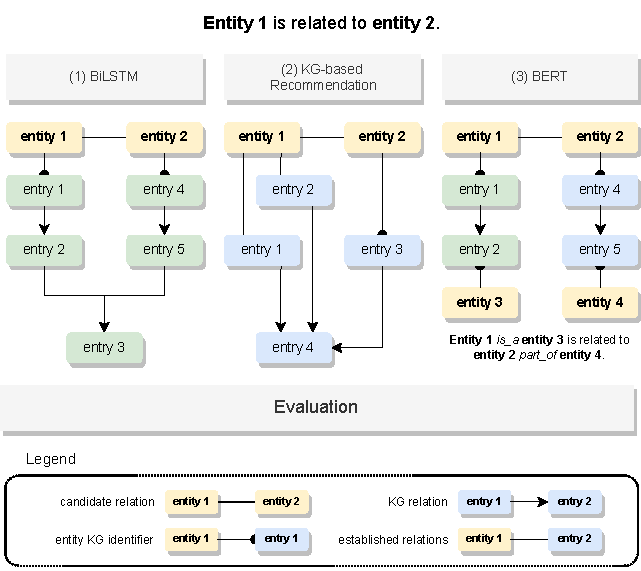
\includegraphics[width=\linewidth]{images/chapter_1/general_metodology.pdf}
\caption[Overview of the General Methodology]{Overview of the methodology followed to accomplish each defined objective. (1) BiLSTMs are a type of RNN composed of multiple layers, which can include entity annotation layers. These annotation layers link each entity to its ontology identifier. In the example, \textit{entity 1} corresponds to \textbf{entry 1} and \textit{entity 2} corresponds to \textbf{entry 4}. Then, we can go through the ontology until we find a common ancestor between the two entities (\textbf{entry 3}), reinforcing the candidate relation. (2) Knowledge Graph (KG)-based recommendation systems have shown the importance of external sources of knowledge to add additional features to items. In the example, knowing that there is a relation between \textit{entity 1} (user) and two other entities represented by \textbf{entry 1} and \textbf{entry 2} (items), that those items link to an \textbf{entry 4} in a KG and that \textit{entity 2} has the identifier \textbf{entry 3} that also links to \textbf{entry 4}, we can reinforce the candidate relation between \textit{entity 1} and \textit{entity 2}. (3) BERT is a language representation model that can be fine-tuned with just one additional output layer, making it possible to integrate the knowledge base data directly into the text where the candidate entities are mentioned. In the example, knowing that \textit{entity 1} has the identifier \textbf{entry 1} and \textit{entity 3} has the identifier \textbf{entry 2}, and that these identifiers are connected in a KG, we can directly integrate this knowledge in the text training data.} \label{fig1}
\end{figure}

\section{Contributions}

The main contributions of this thesis are the biomedical RE text mining solutions developed with added external biomedical knowledge and their evaluation through different approaches. The main chapters of this thesis consist of published articles written in the course of the doctoral work. All systems and datasets are available in open access through the links provided below. 

\subsection{Introductory Book Chapters}

Chapter 2 reflects the contents of two review articles regarding neural networks for relation extraction and text mining using biomedical literature.

\begin{itemize}
    \item{\textbf{Sousa, D.}, Lamurias, A., and Couto, F. M. (2021). \textbf{Using Neural Networks for Relation Extraction from Biomedical Literature}. In Artificial Neural Networks, pages 289–305. Springer, New York, NY, USA. (Q3 Scimago) \citep{sousa2021using}}
\end{itemize}

\begin{itemize}
    \item{Lamurias, A., \textbf{Sousa, D. F.}, and Couto, F. M. (2023). \textbf{Text Mining for Bioinformatics Using Biomedical Literature}. In Encyclopedia of Bioinformatics and Computational Biology. (Accepted) [\hyperlink{AB}{Appendix B}}] 
\end{itemize}

\subsection{Systems}

Chapters 3, 4, and 5 correspond to research articles that reflect the progression of the field of deep learning architectures throughout the doctoral work. Thus, each of the three articles describes a deep learning biomedical RE system, entitled BiOnt, K-BiOnt, and K-RET, respectively. BiOnt and K-RET bypassed the previous state-of-the-art by about 4\% and 3\% in average F-measure, respectively. While K-BiOnt retrieved more rare relations (i.e., complex to identify) than its predecessors. These systems correspond to Objective 1. 

\begin{itemize}
    \item{\textbf{Sousa, D.} and Couto, F. M. (2020). \textbf{BiOnt: Deep Learning Using Multiple Biomedical Ontologies for Relation Extraction}. In Advances in Information Retrieval: 42\textsuperscript{nd} European Conference on IR Research, pages 367–374, Lisbon, Portugal. Springer. (Core A) \citep{sousa2020biont}} \footnote{\url{https://github.com/lasigeBioTM/BiOnt}}
\end{itemize}

\begin{itemize}
    \item{\textbf{Sousa, D.} and Couto, F. M. (2022). \textbf{Biomedical Relation Extraction with Knowledge Graph-based Recommendations}. IEEE Journal of Biomedical and Health Informatics, 26(8):4207–4217. (Q1 Scimago) \citep{sousa2022biomedical}} \footnote{\url{https://github.com/lasigeBioTM/K-BiOnt}}
\end{itemize}

\begin{itemize}
    \item{\textbf{Sousa, D. F.} and Couto, F. M. (2023). \textbf{K-RET: Knowledgeable Biomedical Relation Extraction System}. Bioinformatics, 39(4):1-8. (Q1 Scimago) \citep{sousa2023k}} \footnote{\url{https://github.com/lasigeBioTM/K-RET}}
\end{itemize}

\subsection{Evaluation}

Chapter 6 corresponds to a research article that presents the usage of distant supervision techniques with crowdsourcing platforms to facilitate the creation of biomedical RE datasets. This work resulted in an average F-measure increase of about 35\% compared to relying solely on distant supervision when tested with two state-of-the-art systems. This approach corresponds to Objective 2. 

\begin{itemize}
    \item{\textbf{Sousa, D.}, Lamurias, A., and Couto, F. M. (2020). \textbf{A Hybrid Approach Toward Biomedical Relation Extraction Training Corpora: Combining Distant Supervision with Crowdsourcing}. Database, 2020:1-15. (Q1 Scimago) \citep{sousa2020hybrid}} \footnote{\url{https://github.com/lasigeBioTM/PGR-crowd}}
\end{itemize}

\subsection{Real-World Assessments}

Chapter 7 presents an overview of the work developed regarding workshops, challenges, and topic-adjacent journal contributions, such as participation in SemEval and BioCreative RE-specific community challenges. These contributions were deemed real-world assessments of the systems and approaches developed in this thesis, all corresponding to at least one of the two objectives in some capacity. 

\begin{itemize}
    \item{\textbf{Sousa, D.}, Lamurias, A., and Couto, F. M. (2020). \textbf{Improving Accessibility and Distinction Between Negative Results in Biomedical Relation Extraction}. Genomics \& Informatics, 18(2):1-4. \citep{sousa2020improving}} \footnote{\url{https://github.com/lasigeBioTM/blah6}}
\end{itemize}

\begin{itemize}
    \item{Lamurias, A., \textbf{Sousa, D.}, and Couto, F. M. (2020). \textbf{Generating Biomedical Question Answering Corpora From Q\&A Forums}. IEEE Access, 8:161042–161051. (Q1 Scimago) \citep{lamurias2020generating}} \footnote{\url{https://github.com/lasigeBioTM/BiQA}}
\end{itemize}

\begin{itemize}
    \item{Barros, M., Lamurias, A., \textbf{Sousa, D.}, Ruas, P., and Couto, F. M. (2020). \textbf{COVID-19: A Semantic-Based Pipeline for Recommending Biomedical Entities}. In Proceedings of the 1\textsuperscript{st} Workshop on NLP for COVID-19 (Part 2) at EMNLP 2020, pages 1–9, Online. Association for Computational Linguistics. (Core A) \citep{barros2020covid}} \footnote{\url{https://github.com/lasigeBioTM/knowledge-extraction-from-CORD-19}}
\end{itemize}

\begin{itemize}
    \item{\textbf{Sousa, D.}, Cassanheira, R., and Couto, F. M. (2021). \textbf{lasigeBioTM at BioCreative VII Track 1: Text Mining Drug and Chemical-Protein Interactions Using Biomedical Ontologies}. In Proceedings of the BioCreative VII Challenge Evaluation Workshop, pages 1–4, Online. Association for Computational Linguistics. \citep{sousalasigebiotm}} \footnote{\url{https://github.com/lasigeBioTM/biocreativeVII}}
\end{itemize}

\begin{itemize}
    \item{\textbf{Sousa, D.} (2021). \textbf{Deep Learning System for Biomedical Relation Extraction Combining External Sources of Knowledge}. In Advances in Information Retrieval: 43\textsuperscript{rd} European Conference on IR Research, pages 688–693, Berlin, Heidelberg. Springer. (Core A) \citep{sousa2021deep}}
\end{itemize}

\begin{itemize}
    \item{Barros, M.\footnote[*]{Authors contributed equally to this research}, Ruas, P.\textsuperscript{*}, \textbf{Sousa, D.}\textsuperscript{*}, Bangash, A. H., and Couto, F. M. (2021). \textbf{COVID-19 Recommender System Based on an Annotated Multilingual Corpus}. Genomics \& Informatics, 19(3):1-7. \citep{barros2021covid}} \footnote{\url{https://github.com/lasigeBioTM/blah7}}
\end{itemize} 

\begin{itemize}
    \item{Conceição S. I. R., \textbf{Sousa, D. F.}, Silvestre, P. M., and Couto, F. M. (2023). \textbf{lasigeBioTM at SemEval-2023 Task 7: Improving Natural Language Inference Baseline Systems with Domain Ontologies}. (Accepted)} \footnote{\url{https://github.com/lasigeBioTM/SemEval2023_Task-7}}
\end{itemize}

\begin{itemize}
    \item{Ruas, P.\footnote[†]{Authors contributed equally to this research}, \textbf{Sousa, D. F.}\textsuperscript{†}, Neves, A.\textsuperscript{†}, Cruz, C., and Couto, F. M. (2023). \textbf{LASIGE and UNICAGE Solution to the NASA LitCoin NLP Competition}. (Submitted) (7\textsuperscript{th} Place in the NASA LitCoin NLP Challenge with cash prize of 5.000 USD)} \footnote{\url{https://github.com/lasigeBioTM/Litcoin-Lasige_Unicage}}
\end{itemize}

\section{Document Structure}

In addition to the present introductory chapter, this document is structured into eight chapters as follows:

\begin{itemize}
   \item \textbf{Chapter \hyperlink{2}{2}} (Biomedical Relation Extraction) provides an overview of the key concepts to understand biomedical RE according to the two main objectives established previously. 
   \item \textbf{Chapter \hyperlink{3}{3}} (BiOnt: Deep Learning Using Multiple Biomedical Ontologies for Relation Extraction) presents the BiOnt system, a BiLSTM-based system with annotation layers based on biomedical ontologies. 
   \item \textbf{Chapter \hyperlink{4}{4}} (Biomedical Relation Extraction with Knowledge Graph-based Recommendations) showcases the K-BiOnt system. This system joins the abilities of KG-based recommendation systems and BiOnt by defining biomedical entities as items and ontological KG annotations as features. 
   \item \textbf{Chapter \hyperlink{5}{5}} (K-RET: Knowledgeable Biomedical Relation Extraction System) presents the K-RET system, a BERT-based system with added biomedical knowledge in the form of text expansion in the fine-tuning stage. 
   \item \textbf{Chapter \hyperlink{6}{6}} (A Hybrid Approach toward Biomedical Relation Extraction Training Corpora: Combining Distant Supervision with Crowdsourcing) demonstrates how to combine distant supervision approaches with crowdsourcing to boost the creation of biomedical RE datasets. 
   \item \textbf{Chapter \hyperlink{7}{7}} (Real-World Assessments) compiles all other research work conducted throughout this thesis by dividing each contribution into a section summarising its motivation and the work developed. 
   \item \textbf{Chapter \hyperlink{8}{8}} (General Discussion and Conclusions) closes the thesis by presenting a general discussion of the thesis, its main conclusions, and future work.
\end{itemize}